\chapter{HISTORY OF MONEY}
\label{ch:historyofmoney}

How did we get here? How do we transfer value, and how did we do this in the past? When you think about it, what is currency and what is money? Throughout history, people exchanged value from one person to another through trade, bartering, exchange of goods and services but mostly by using something we call money. The crisis of 2008 showed us how vulnerable the current monetary system is. The current system is inherently flawed, debt-based and unsustainable. It benefits the few, not the many. If and when distributed ledger technology is implemented for the greater good, the potential for disruption is massive, particularly in the financial services industry. Before we go there, let's first discuss the history of money, fiat currency and the current monetary system and policies of today.

\bigskip
\bigskip
\tcbset{colback=orange!3!white,fonttitle=\bfseries}
    \begin{tcolorbox}
    [enhanced,
    title=All Fiat Currencies become Worthless,
    frame style=
    {left color=orange!85!black,right color=yellow!95!black}]
    
      
Through recorded history, no fiat currency has survived, all fiat currencies that ever  existed  ended up with an intrinsic value of zero 
 \parencite{thebigreset}.
\end{tcolorbox}
\bigskip

\section{Properties of money}
Money  dates back to thousands of years. However, the money we have and use today is very different from the money we  had in the past. Let's look at some of the most important properties of sound money as defined by  worldwide bestselling author and internationally renowned expert on the history of money, Mike Maloney. In his book Guide to Investing in Gold \& Silver: Protect your Financial Future, Mike states that the following characteristics define sound money:

\begin{enumerate}[label=(\alph*)]
    \setlength\itemsep{0em}
    \item Money is a medium of exchange
    \item Money is a unit of account
    \item Money is durable and does not spoil or corrode
    \item Money is portable
    \item Money is divisible
    \item Money is fungible (each unit is interchangeable)
    \item \textbf{Money is a true store of value over time}
\end{enumerate}

\section{Sound money}
The first sound money system which was used in any known civilization was based on physical gold and silver. Pure, minted coins ensured that governments, unilateral organizations and bankers were kept in check as they could not create new currency out of thin air. A currency was either sound money or backed by sound money. In the case of civilizations that used real gold and silver coins, problems only occurred after  governments started  debasing their coinage, meaning melting down your currency and adding an inferior base metal to increase the total coin supply \cite{goldsilver ep2}.


\subsection{Store of value over time}

The supply of gold is finite, effectively making it a scarce resource, both historically and today. It has and will always be necessary for people that money maintains its store of value over time. Assuring store of value over a long period is a prime example of what makes a commodity such as gold sound money. To top this off, nobody can produce or create more gold out of thin air, unlike the debt-based fiat currency based system we know today.

\begin{quotation}

      \textit{\say{In 500 BC, you could buy a Roman senator's Toga for one ounce of gold, you could purchase a Brooks Brothers suit in the 19th century for one ounce of gold, and today a new Italian suit is worth one ounce of gold.}}
      \begin{flushright}
        \small{--- \textbf{R.W. Jastram}}
      \end{flushright}
    
\end{quotation}

\section{Fake Money, Fake System}
Unfortunately, today, countries no longer back up their currencies with commodities. For example, let's look at the pounds sterling (\pounds) and the U.S. dollar (US\$), which we know as money today but are, in fact, just currencies.\medskip

The inherent flaws of the capitalist system have led us through several business and financial cycles that have resulted in the so-called \say{booms} and \say{busts} in asset prices. Ever since the \$USD went off the gold-standard in 1971, there  have been no restrictions  in terms of the money supply as it is no longer backed by sound money. Eventually, this leads to a situation where financial products, which add no value to the economy, are created exponentially.

In the process, intermediaries, middlemen and banks, who are the creators of those debt products, have made much profit and have simultaneously created an enormous amount of debt. Moreover, as financial products increase, the ratio of money that goes to products or services that add value to the economy and society is decreasing. The financial sector is booming, as there are no restrictions regarding the money supply, which allows them to conjure  up credit out of thin air in forms of debts and loans and make money off interests. Debt is the product of the financial industry, and debt is how they are making a killing.


\tcbset{colback=orange!3!white,fonttitle=\bfseries}
    \begin{tcolorbox}
    [enhanced,
    title=Nixon shock - off the gold standard,
    frame style=
    {left color=orange!85!black,right color=yellow!95!black}]
    
      Since the United States cancelled the convertibility of the US\$ to gold with the "Nixon Shock" in the 70s, national currencies have had freely floating exchange rates. Central banks' monetary policies have mainly dictated these rates. In 1971, the Nixon administration took the international dollar off the gold standard and from this moment the U.S. reverted to a system which depended only on fiat currency where the US\$ was backed only by debts and promises. 
\end{tcolorbox}
\medskip

This decision still affects the world today because the US\$ was - and still is - the global reserve currency. Ever since, banks and financial intermediaries but also as well as currency creators, such as the U.S. Federal Reserve, Bank of Japan, European Central Bank (ECB) and Bank of China have had a lot of control and influence over the money supply.

\section{Fiat currency}       
Fiat currency is a currency that exists at the dictate or by fiat from a government (fiat is a Latin word for a currency that is circulating by force). Fiat currencies are indeed abundant and widely available within the jurisdictions where they are accepted. Modern paper money and coins, along with their digital counterparts, are durable enough; however, fiat money can no longer claim to have any intrinsic value. Its value is perceived based on faith, and that faith originates from the respective government backing and a national or international trust in the stability of the currency.

No government or bank has ever been able to discipline its monetary policy. History has shown that implementing a fiat currency model makes it easier for any government to do any of the following (there is no limit since the currency itself has no intrinsic value and is unbacked by sound money such as gold);

\begin{enumerate}[label=(\alph*)]
    \setlength\itemsep{0em}
    \item Increase the money supply through borrowing
    \item Increase the money supply through simply printing
    \item Increase spending (the particularly harmful deficit spending of currency we don't have)
    \item Impose burdensome regulations on small businesses and implement monetary policies to expand its control further
\end{enumerate}

\noindent Throughout history, no fiat currency has ever survived, and all fiat currencies that have ever existed went to a value of zero\cite{fiattozero1, fiattozero2}. If you compare this to gold, this is entirely different. It doesn't matter if a gold coin has a value of \$120 or \$15000. The value lies in what real goods or services you can buy with it, not the absolute value expressed in some (national) fiat currency.

\begin{quotation}

      \textit{\say{Paper money eventually returns to its intrinsic value - zero.}}
      \begin{flushright}
        \small{--- \textbf{Voltaire}}
      \end{flushright}
    
\end{quotation}

\section{Purchasing power}
Comparing gold to any fiat currency is like comparing apples to oranges. This is the same if we talk about paper fiat currency (cash) or digital fiat currency (on your bank account).  Fiat currency meets two of the conditions of 'real money': it is a unit of account and a medium of exchange. However, fiat currency isn't a store of value over a long period.  Any fiat currency created by any government tends to lose value over time for several reasons. One of them is inflation. Inflation is the result of too much money chasing insufficient goods, which makes your fiat currency depreciate as the money supply expands. 

For example, an inflation rate of more than 2\% per year, which is common nowadays in the western world, cuts your savings in terms of what you can buy with it (purchasing power) in half in 25 years. Without taking into account the consumer inflation for products; the same price for smaller quantities of the same product. Inflation occurs over a very long time, and many people do not realize that their currency is slowly but surely becoming worthless - like a time bomb set to explode. When the fiat currency based economy finally collapses after so many rounds of quantitative easing and hyperinflation kicks in - the results are usually catastrophic\cite{weimarhyperinflation}. \medskip

\medskip

    \tcbset{colback=orange!3!white,fonttitle=\bfseries}
    \begin{tcolorbox}
    [enhanced,
    title=Banking system,
    frame style=
    {left color=orange!85!black,right color=yellow!95!black}]

         \itshape{The rules of money and banking have changed every 20 or 30 years for the past three centuries, in an ongoing trial-and-error experiment in evolving a financial system, and a constant battle over whose interests it will serve. Presenting that timeline in full will take another article, but in a nutshell, we have gone from precious metal coins to government-issued paper script, privately-issued banknotes, chequebook money, gold-backed Federal Reserve Notes, unbacked Federal Reserve Notes, and the \say{near money} created by the shadow banking system. Money has evolved from being \say{stored} in the form of a physical commodity to paper representations of value, to computer bits storing information about credits and debits.}
        
        \tcblower
        
        \textbf{The rules have been changed before and can be changed again.} Depressions, credit crises and financial collapse are not acts of God but induced by mechanical flaws or corruption in the financial system. Credit may stop flowing, but the workers, materials and markets are still there. The system needs a reboot. Hopefully, the next program that gets run will last more than 20 or 30 years. Ideally, we might mimic the ancient Mesopotamians, the oldest and most long-lasting civilization in history, and devise an economic system that lasts for millennia.\cite{EllenBrown}

\end{tcolorbox}

\medskip

\noindent When the world went off the gold standard, central banks and governments were not accountable to anybody or forced to restrict the money supply (as it was not pegged to something with real value anymore). Not having the requirement in place to back printed money with a physical asset has led to an explosion of debt in the financial sector. The financial industry now transacts trillions in a range of financial products, its effects are visible in many economic indicators.\medskip

\section{Questionable monetary policy}
Several other factors and parties destroy the purchasing power of the fiat currency. Once a government has introduced a fiat currency, it usually can't resist the temptation of expanding the currency supply through deficit spending (increasing the public debt ceiling). Commercial banks are creating money out of thin air by fractional reserve banking. Central banks are creating money by providing loans to governments and commercial banks. On top of this, since 2008, almost all central banks all over the world such as the European Central Bank, Federal Reserve, Bank of England and the People's Bank of China have been executing the policy of what they call Quantitative Easing (QE). QE is an expansionary monetary policy whereby a central bank buys predetermined amounts of government bonds or other financial assets to stimulate the economy and increase liquidity. An unconventional form of monetary policy, it is usually used when inflation is very low or negative, and standard expansionary monetary policy has become ineffective.

This policy is nothing more than a process where the authoritative body injects an insane quantity of currency into the economy at near zero percent interest rates to serve as a stimulus for the economy. Ultimately, it's just more debt. Refer to \cref{fig:fedgraph_debt_EU,fig:fedgraph_debt_US,fig:fedgraph_debt_JPN} for an impression of ever-increasing debt levels (as a \% of GDP) for the US, EU and Japan. There are now many countries around the world where this policy is applied.




    \begin{figure}
        \centering
        \caption{Central Government debt, total \% of GDP for the Euro Area}
        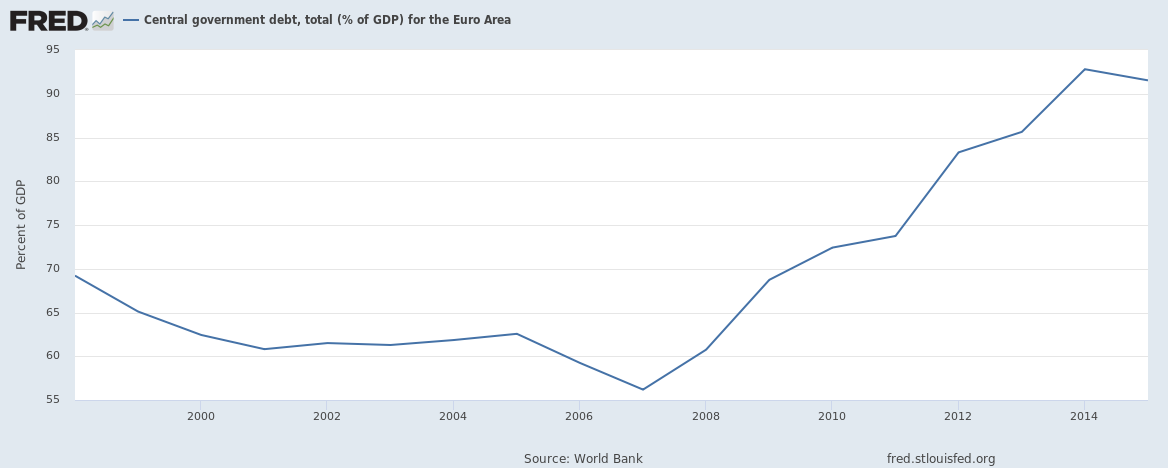
\includegraphics[width=\textwidth]{img/ch-history/fredgraph_debt_EU.png}
       
        \label{fig:fedgraph_debt_EU}
        \source{Federal Reserve Bank of St. Louis, Economic Research \cite{FRED}}
    \end{figure}
    
    \begin{figure}
        \centering
        \caption{Federal Government total public debt as a \% of GDP for the US}
        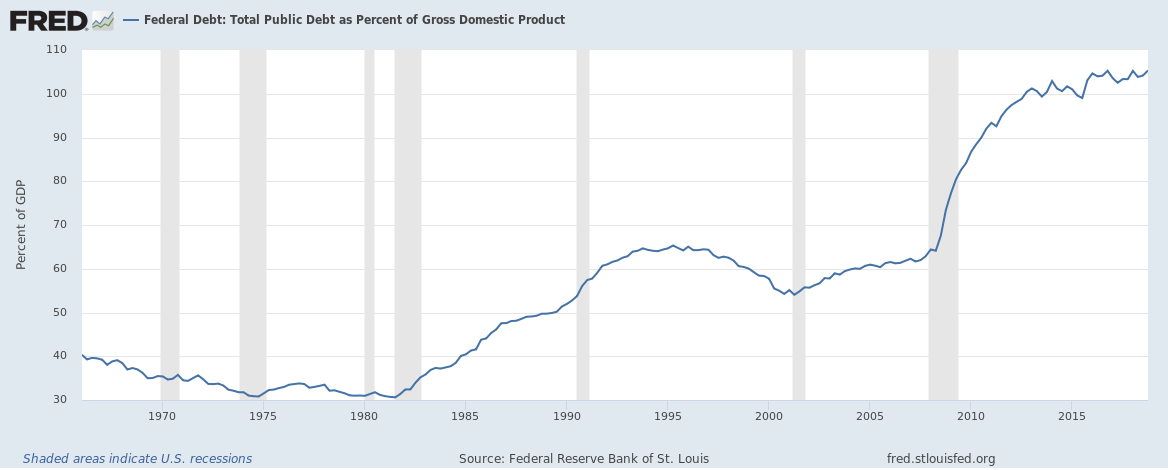
\includegraphics[width=\textwidth]{img/ch-history/fredgraph_debt_US.png}
       
        \label{fig:fedgraph_debt_US}
        \source{Federal Reserve Bank of St. Louis, Economic Research \cite{FRED}}
    \end{figure}
    
    \begin{figure}
        \centering
        \caption{Central Government debt, total \% of GDP for Japan}
        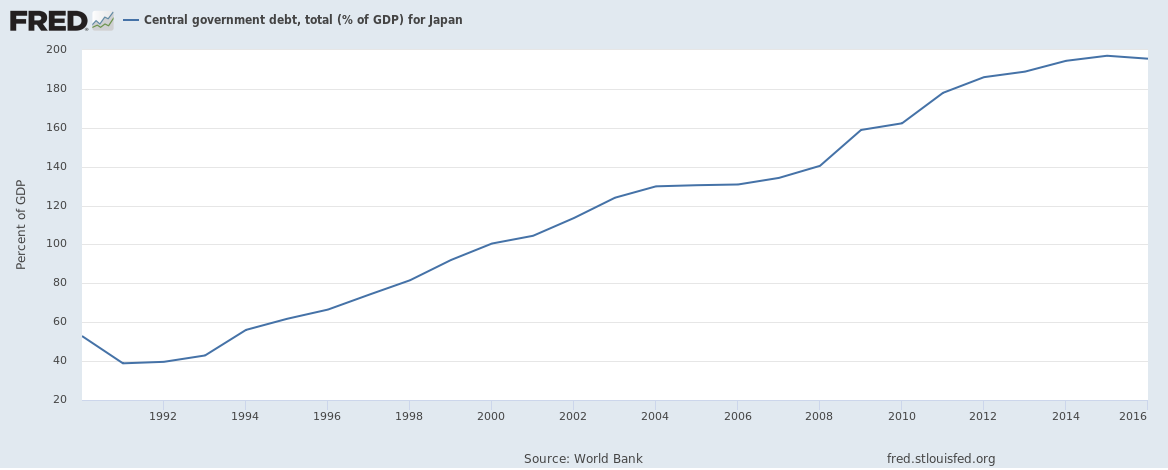
\includegraphics[width=\textwidth]{img/ch-history/fredgraph_debt_JPN.png}
       
        \label{fig:fedgraph_debt_JPN}
        \source{Federal Reserve Bank of St. Louis, Economic Research \cite{FRED}}
    \end{figure}

\section{Post financial crisis 2008}
        
The result was an even more gigantic debt bubble that heralded the financial crisis of '08. Inevitably, when interest rates are going to rise again, the lion's share of all debtors will have immense problems paying off their debts plus added interest.\medskip 


\begin{quotation}

      \textit{\say{In 2000, we had the dot-com bubble. In 2008, we had the housing bubble. In 2020, we had the \emph{everything} bubble}}
      \begin{flushright}
        \small{--- \textbf{Mauldin Economics}}
      \end{flushright}
    
\end{quotation}

In the previous financial crashes, central banks had an opportunity to stimulate the economy by lowering interest rates, which made capital less expensive so people could lend more. Ten years after the last crash, interest rates are still near zero. Having interest close to zero provides very little to no room for lowering interest rates (again) and 'save' us from yet another depression. In 2008, they just delayed the inevitable, but in the future, we will have to deal with the consequences.\medskip

On top of this, by creating enormous amounts of fiat currency, the money supply expands, and more currency is chasing the same amount of goods and services, which results in high inflation rates. High inflation rates result in higher prices for products and services. Moreover, eventually, when all fiat (digital) currency is circulating in the economy, it could result in a global fiat currency crisis through hyperinflation. \Cref{tab:inflationratescountries} shows countries with high inflation rates and note that Venezuela suffers from severe hyperinflation. Such an event has the potential to obliterate the saving accounts of entire generations, and all of our currency suddenly becomes worthless paper. 

\begin{table}
\centering
\caption{Inflation rates $>$ 20\%}
\begin{tabular}{@{}llll@{}}
\toprule
\textbf{Country} & \multicolumn{3}{l}{\textbf{Inflation rates {[}\%{]}}} \\ 
\textbf{}        & Q4 ''18          & Q1 ''19          & Q2 ''19         \\ \midrule
Venezuela        & 1698488          &                  & 282973          \\
Argentina        & 47.1             &                  & 57.3            \\
Sudan            &                  & 43.5            & 44.6            \\
South Sudan      & 33.5             &                  & 56.1            \\
Zimbabwe         & 42.1             &                  & 97.9           \\
Iran             & 39.9             &                  & 52.2            \\
Liberia          & 26.6             &                  & 23.3            \\
Turkey           &                  & 20.4            & 18.7           \\ \bottomrule
\end{tabular}
\source{Trading Economics. \emph{Inflation Rate - World.} \cite{tradingeconomics}}
\label{tab:inflationratescountries}
\end{table}


\noindent In short, the history of fiat currencies is a history of volatility. The average lifespan of a fiat currency is only twenty-seven (27) years. Even if a currency survives any longer, invariably it will experience increasing inflation. Inflation steadily erodes the purchasing power of fiat money over time. The world's oldest fiat currency, the British pound (\pounds), is an excellent example; it has lost ninety-nine and a half per cent (99.5\%) of its value since inception. Historically gold is more resilient, and holds its value better than any fiat currency and is particularly strong in times of economic instability.

\begin{quotation}

  \textit{\say{In the midst of every crisis, lies great opportunity.}}
  \begin{flushright}
    \small{--- \textbf{Einstein, Albert}}
  \end{flushright}

\end{quotation}

\section{Legacy financial infrastructures}

At present, we mostly rely on middlemen or intermediaries like banks, commerce platforms or governments to establish the element that allows our economy to function in a digitized space: trust. These third parties perform transactional logistics like authentication, record-keeping or payment clearance to ensure that both parties in a transaction oblige to some pre-specified terms and conditions, and thus allowing the buyer and seller to remain confident that the transaction will be executed securely and effectively.
While these intermediaries are crucial to our digital economy, there are some significant issues.

\begin{itemize}
    \setlength\itemsep{0em}

    \item They use centralized databases which face high risks of being hacked
    \item They exclude billions of people, who lack access to resources and capital, from the global economy
    \item They charge transaction fees in the form of hefty commissions, not to mention the major timing inefficiencies
    \item They undermine the privacy of the users when they track and use our data as a function of their marketing efforts and business model
    \item They have appropriated the largest of the digital age asymmetrically, as we have wealth creation but growing economic and social inequality
\end{itemize}

\begin{quote}
    \textbf{\emph{Enter the New World of Blockchain}}
\end{quote}
